\section*{Problem 2: findRange} 


\textbf{a)} Betrachten Sie den folgenden binären Suchbaum:
\noindent
Wo befinden sich die Schlüssel, die kleiner sind als 37? Wo befinden sich die
Schlüssel, die größer sind als 21? Wo befinden sich die Schlüssel, die zwischen
21 und 37 liegen?

\begin{center}
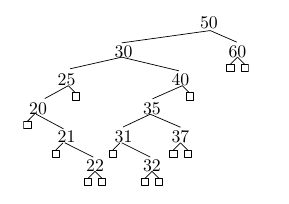
\includegraphics[scale=1]{Aufgabe2}
\end{center}


\textbf{Knoten $<$ 37:}
\begin{itemize}
\item Alle Knoten, die von den 37 Knoten im Baum übrig bleiben (visuell)
\item Knoten 30 und der gesamte linke Teilbaum von 30 und der linke Teilbaum von 40 (ohne 37 selbst)
\item Knoten $<$ 37 umfassen: $\{30, 25, 20, 21, 22, 35, 31, 32\}$
\end{itemize}


\textbf{Knoten $>$ 21:}
\begin{itemize}
\item Alle Knoten rechts vom 21. Knoten im Baum (visuell)
\item Alle Vorgänger Knoten des Knoten 21, für die gilt: $n > 21$
\item Die rechten Teilbäume dieser Vorgänger
\item Knoten $>$ 21: {22, 25, 30, 40, 35, 31, 32, 37, 50, 60}
\end{itemize}


\textbf{Knoten $>$ 21 und Knoten $<$ 37:}
\begin{itemize}
\item Alle Knoten, die visuell links von 37 und rechts von 21 sind.
\item Knoten im rechten Teilbaum von 21
\item Der Knoten 30 und alle Knoten des linken Teilbaums von 30, für die vergoldeten $n > 21$
\item Knoten im linken Teilbaum von 40 außer dem Knoten 37 selbst.
\item \textbf{Knoten $>$ 21 und Knoten $<$ 37:} {22, 25, 30, 31, 32, 35}
\end{itemize}


\newpage
\noindent
\textbf{b)} Beschreiben Sie, wie man in einem AVL-Baum mit $n$ Schlüsseln die Operation
findRange(k1 , k2 ) implementieren kann, die alle Schlüssel $k$ liefert, für die
$k1 \leq k \leq k2$ ist. Die Laufzeit soll $O(log n + s)$ betragen. Dabei ist s die Anzahl
der gelieferten Schlüssel.




 







